\documentclass{standalone}
\usepackage{tikz-feynman}

\begin{document}
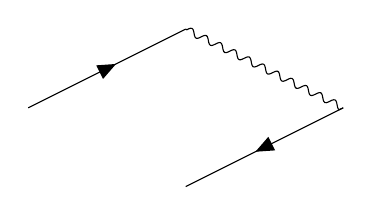
\begin{tikzpicture}
    \begin{feynman}
        \vertex (a) at (-2,0);
        \vertex (b) at (0,1);
        \vertex (c) at (2,0);
        \vertex (d) at (0,-1);

        \diagram* {
            (a) -- [fermion] (b),
            (b) -- [photon] (c),
            (c) -- [fermion] (d),
        };
    \end{feynman}
\end{tikzpicture}
\end{document}